\documentclass[1p]{elsarticle_modified}
%\bibliographystyle{elsarticle-num}

%\usepackage[colorlinks]{hyperref}
%\usepackage{abbrmath_seonhwa} %\Abb, \Ascr, \Acal ,\Abf, \Afrak
\usepackage{amsfonts}
\usepackage{amssymb}
\usepackage{amsmath}
\usepackage{amsthm}
\usepackage{scalefnt}
\usepackage{amsbsy}
\usepackage{kotex}
\usepackage{caption}
\usepackage{subfig}
\usepackage{color}
\usepackage{graphicx}
\usepackage{xcolor} %% white, black, red, green, blue, cyan, magenta, yellow
\usepackage{float}
\usepackage{setspace}
\usepackage{hyperref}

\usepackage{tikz}
\usetikzlibrary{arrows}

\usepackage{multirow}
\usepackage{array} % fixed length table
\usepackage{hhline}

%%%%%%%%%%%%%%%%%%%%%
\makeatletter
\renewcommand*\env@matrix[1][\arraystretch]{%
	\edef\arraystretch{#1}%
	\hskip -\arraycolsep
	\let\@ifnextchar\new@ifnextchar
	\array{*\c@MaxMatrixCols c}}
\makeatother %https://tex.stackexchange.com/questions/14071/how-can-i-increase-the-line-spacing-in-a-matrix
%%%%%%%%%%%%%%%

\usepackage[normalem]{ulem}

\newcommand{\msout}[1]{\ifmmode\text{\sout{\ensuremath{#1}}}\else\sout{#1}\fi}
%SOURCE: \msout is \stkout macro in https://tex.stackexchange.com/questions/20609/strikeout-in-math-mode

\newcommand{\cancel}[1]{
	\ifmmode
	{\color{red}\msout{#1}}
	\else
	{\color{red}\sout{#1}}
	\fi
}

\newcommand{\add}[1]{
	{\color{blue}\uwave{#1}}
}

\newcommand{\replace}[2]{
	\ifmmode
	{\color{red}\msout{#1}}{\color{blue}\uwave{#2}}
	\else
	{\color{red}\sout{#1}}{\color{blue}\uwave{#2}}
	\fi
}

\newcommand{\Sol}{\mathcal{S}} %segment
\newcommand{\D}{D} %diagram
\newcommand{\A}{\mathcal{A}} %arc


%%%%%%%%%%%%%%%%%%%%%%%%%%%%%5 test

\def\sl{\operatorname{\textup{SL}}(2,\Cbb)}
\def\psl{\operatorname{\textup{PSL}}(2,\Cbb)}
\def\quan{\mkern 1mu \triangleright \mkern 1mu}

\theoremstyle{definition}
\newtheorem{thm}{Theorem}[section]
\newtheorem{prop}[thm]{Proposition}
\newtheorem{lem}[thm]{Lemma}
\newtheorem{ques}[thm]{Question}
\newtheorem{cor}[thm]{Corollary}
\newtheorem{defn}[thm]{Definition}
\newtheorem{exam}[thm]{Example}
\newtheorem{rmk}[thm]{Remark}
\newtheorem{alg}[thm]{Algorithm}

\newcommand{\I}{\sqrt{-1}}
\begin{document}

%\begin{frontmatter}
%
%\title{Boundary parabolic representations of knots up to 8 crossings}
%
%%% Group authors per affiliation:
%\author{Yunhi Cho} 
%\address{Department of Mathematics, University of Seoul, Seoul, Korea}
%\ead{yhcho@uos.ac.kr}
%
%
%\author{Seonhwa Kim} %\fnref{s_kim}}
%\address{Center for Geometry and Physics, Institute for Basic Science, Pohang, 37673, Korea}
%\ead{ryeona17@ibs.re.kr}
%
%\author{Hyuk Kim}
%\address{Department of Mathematical Sciences, Seoul National University, Seoul 08826, Korea}
%\ead{hyukkim@snu.ac.kr}
%
%\author{Seokbeom Yoon}
%\address{Department of Mathematical Sciences, Seoul National University, Seoul, 08826,  Korea}
%\ead{sbyoon15@snu.ac.kr}
%
%\begin{abstract}
%We find all boundary parabolic representation of knots up to 8 crossings.
%
%\end{abstract}
%\begin{keyword}
%    \MSC[2010] 57M25 
%\end{keyword}
%
%\end{frontmatter}

%\linenumbers
%\tableofcontents
%
\newcommand\colored[1]{\textcolor{white}{\rule[-0.35ex]{0.8em}{1.4ex}}\kern-0.8em\color{red} #1}%
%\newcommand\colored[1]{\textcolor{white}{ #1}\kern-2.17ex	\textcolor{white}{ #1}\kern-1.81ex	\textcolor{white}{ #1}\kern-2.15ex\color{red}#1	}

{\Large $\underline{12n_{0600}~(K12n_{0600})}$}

\setlength{\tabcolsep}{10pt}
\renewcommand{\arraystretch}{1.6}
\vspace{1cm}\begin{tabular}{m{100pt}>{\centering\arraybackslash}m{274pt}}
\multirow{5}{120pt}{
	\centering
	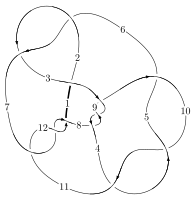
\includegraphics[width=112pt]{../../../GIT/diagram.site/Diagrams/png/2689_12n_0600.png}\\
\ \ \ A knot diagram\footnotemark}&
\allowdisplaybreaks
\textbf{Linearized knot diagam} \\
\cline{2-2}
 &
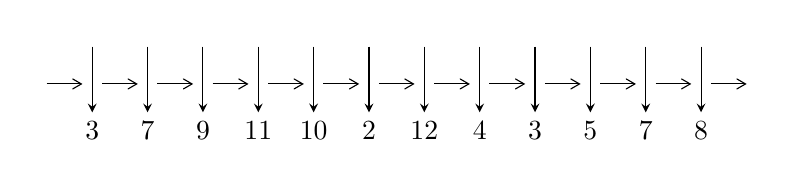
\begin{tikzpicture}[x=20pt, y=17pt]
	% nodes
	\node (C0) at (0, 0) {};
	\node (C1) at (1, 0) {};
	\node (C1U) at (1, +1) {};
	\node (C1D) at (1, -1) {3};

	\node (C2) at (2, 0) {};
	\node (C2U) at (2, +1) {};
	\node (C2D) at (2, -1) {7};

	\node (C3) at (3, 0) {};
	\node (C3U) at (3, +1) {};
	\node (C3D) at (3, -1) {9};

	\node (C4) at (4, 0) {};
	\node (C4U) at (4, +1) {};
	\node (C4D) at (4, -1) {11};

	\node (C5) at (5, 0) {};
	\node (C5U) at (5, +1) {};
	\node (C5D) at (5, -1) {10};

	\node (C6) at (6, 0) {};
	\node (C6U) at (6, +1) {};
	\node (C6D) at (6, -1) {2};

	\node (C7) at (7, 0) {};
	\node (C7U) at (7, +1) {};
	\node (C7D) at (7, -1) {12};

	\node (C8) at (8, 0) {};
	\node (C8U) at (8, +1) {};
	\node (C8D) at (8, -1) {4};

	\node (C9) at (9, 0) {};
	\node (C9U) at (9, +1) {};
	\node (C9D) at (9, -1) {3};

	\node (C10) at (10, 0) {};
	\node (C10U) at (10, +1) {};
	\node (C10D) at (10, -1) {5};

	\node (C11) at (11, 0) {};
	\node (C11U) at (11, +1) {};
	\node (C11D) at (11, -1) {7};

	\node (C12) at (12, 0) {};
	\node (C12U) at (12, +1) {};
	\node (C12D) at (12, -1) {8};
	\node (C13) at (13, 0) {};

	% arrows
	\draw[->,>={angle 60}]
	(C0) edge (C1) (C1) edge (C2) (C2) edge (C3) (C3) edge (C4) (C4) edge (C5) (C5) edge (C6) (C6) edge (C7) (C7) edge (C8) (C8) edge (C9) (C9) edge (C10) (C10) edge (C11) (C11) edge (C12) (C12) edge (C13) ;	\draw[->,>=stealth]
	(C1U) edge (C1D) (C2U) edge (C2D) (C3U) edge (C3D) (C4U) edge (C4D) (C5U) edge (C5D) (C6U) edge (C6D) (C7U) edge (C7D) (C8U) edge (C8D) (C9U) edge (C9D) (C10U) edge (C10D) (C11U) edge (C11D) (C12U) edge (C12D) ;
	\end{tikzpicture} \\
\hhline{~~} \\& 
\textbf{Solving Sequence} \\ \cline{2-2} 
 &
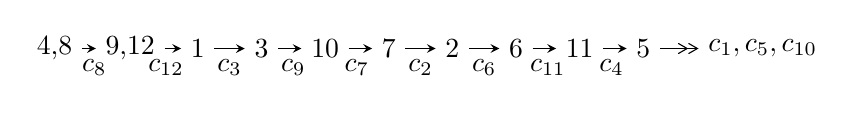
\begin{tikzpicture}[x=23pt, y=7pt]
	% node
	\node (A0) at (-1/8, 0) {4,8};
	\node (A1) at (17/16, 0) {9,12};
	\node (A2) at (17/8, 0) {1};
	\node (A3) at (25/8, 0) {3};
	\node (A4) at (33/8, 0) {10};
	\node (A5) at (41/8, 0) {7};
	\node (A6) at (49/8, 0) {2};
	\node (A7) at (57/8, 0) {6};
	\node (A8) at (65/8, 0) {11};
	\node (A9) at (73/8, 0) {5};
	\node (C1) at (1/2, -1) {$c_{8}$};
	\node (C2) at (13/8, -1) {$c_{12}$};
	\node (C3) at (21/8, -1) {$c_{3}$};
	\node (C4) at (29/8, -1) {$c_{9}$};
	\node (C5) at (37/8, -1) {$c_{7}$};
	\node (C6) at (45/8, -1) {$c_{2}$};
	\node (C7) at (53/8, -1) {$c_{6}$};
	\node (C8) at (61/8, -1) {$c_{11}$};
	\node (C9) at (69/8, -1) {$c_{4}$};
	\node (A10) at (11, 0) {$c_{1},c_{5},c_{10}$};

	% edge
	\draw[->,>=stealth]	
	(A0) edge (A1) (A1) edge (A2) (A2) edge (A3) (A3) edge (A4) (A4) edge (A5) (A5) edge (A6) (A6) edge (A7) (A7) edge (A8) (A8) edge (A9) ;
	\draw[->>,>={angle 60}]	
	(A9) edge (A10);
\end{tikzpicture} \\ 

\end{tabular} \\

\footnotetext{
The image of knot diagram is generated by the software ``\textbf{Draw programme}" developed by Andrew Bartholomew(\url{http://www.layer8.co.uk/maths/draw/index.htm\#Running-draw}), where we modified some parts for our purpose(\url{https://github.com/CATsTAILs/LinksPainter}).
}\phantom \\ \newline 
\centering \textbf{Ideals for irreducible components\footnotemark of $X_{\text{par}}$} 
 
\begin{align*}
I^u_{1}&=\langle 
u^7- u^6+5 u^5-8 u^4+12 u^3-15 u^2+8 b+16 u-6,\;u^6+3 u^4- u^3+u^2+4 a-4 u-2,\\
\phantom{I^u_{1}}&\phantom{= \langle  }u^8+4 u^6-3 u^5+4 u^4-11 u^3+u^2-6 u+2\rangle \\
I^u_{2}&=\langle 
- u^2 a- u^3+b- a- u-1,\;2 u^3 a-2 u^2 a- u^3+2 a^2+2 a u+u^2+2 a-1,\;u^4+u^2+u+1\rangle \\
I^u_{3}&=\langle 
-211 u^9-520 u^8-1473 u^7-2621 u^6-4433 u^5-6682 u^4-6460 u^3-6461 u^2+893 b-3449 u-911,\\
\phantom{I^u_{3}}&\phantom{= \langle  }-3011 u^9-6938 u^8+\cdots+8930 a-4451,\\
\phantom{I^u_{3}}&\phantom{= \langle  }u^{10}+3 u^9+8 u^8+16 u^7+27 u^6+43 u^5+49 u^4+48 u^3+38 u^2+16 u+5\rangle \\
I^u_{4}&=\langle 
- u^5+u^4- u^2 a-2 u^3+2 u^2+b- a-2 u+2,\;2 u^5 a+2 u^3 a+u^4-2 u^2 a- u^3+a^2+a u+u^2-2 a-2 u+2,\\
\phantom{I^u_{4}}&\phantom{= \langle  }u^6- u^5+2 u^4-2 u^3+2 u^2-2 u+1\rangle \\
I^u_{5}&=\langle 
b-1,\;6 a- u-3,\;u^2+3\rangle \\
I^u_{6}&=\langle 
b+u,\;2 a- u+1,\;u^2+1\rangle \\
\\
I^v_{1}&=\langle 
a,\;b-1,\;v+1\rangle \\
\end{align*}
\raggedright * 7 irreducible components of $\dim_{\mathbb{C}}=0$, with total 43 representations.\\
\footnotetext{All coefficients of polynomials are rational numbers. But the coefficients are sometimes approximated in decimal forms when there is not enough margin.}
\newpage
\renewcommand{\arraystretch}{1}
\centering \section*{I. $I^u_{1}= \langle u^7- u^6+\cdots+8 b-6,\;u^6+3 u^4- u^3+u^2+4 a-4 u-2,\;u^8+4 u^6-3 u^5+4 u^4-11 u^3+u^2-6 u+2 \rangle$}
\flushleft \textbf{(i) Arc colorings}\\
\begin{tabular}{m{7pt} m{180pt} m{7pt} m{180pt} }
\flushright $a_{4}=$&$\begin{pmatrix}0\\u\end{pmatrix}$ \\
\flushright $a_{8}=$&$\begin{pmatrix}1\\0\end{pmatrix}$ \\
\flushright $a_{9}=$&$\begin{pmatrix}1\\u^2\end{pmatrix}$ \\
\flushright $a_{12}=$&$\begin{pmatrix}-\frac{1}{4} u^6-\frac{3}{4} u^4+\cdots+u+\frac{1}{2}\\-\frac{1}{8} u^7+\frac{1}{8} u^6+\cdots-2 u+\frac{3}{4}\end{pmatrix}$ \\
\flushright $a_{1}=$&$\begin{pmatrix}\frac{1}{8} u^7-\frac{3}{8} u^6+\cdots+3 u-\frac{1}{4}\\-\frac{1}{8} u^7+\frac{1}{8} u^6+\cdots-2 u+\frac{3}{4}\end{pmatrix}$ \\
\flushright $a_{3}=$&$\begin{pmatrix}u\\u^3+u\end{pmatrix}$ \\
\flushright $a_{10}=$&$\begin{pmatrix}u^2+1\\u^4+2 u^2\end{pmatrix}$ \\
\flushright $a_{7}=$&$\begin{pmatrix}-\frac{1}{4} u^6-\frac{3}{4} u^4+\cdots+u+\frac{1}{2}\\\frac{3}{8} u^7+\frac{1}{8} u^6+\cdots-2 u+\frac{3}{4}\end{pmatrix}$ \\
\flushright $a_{2}=$&$\begin{pmatrix}\frac{1}{4} u^6+\frac{3}{4} u^4+\cdots+\frac{1}{4} u^2+\frac{1}{2}\\-\frac{3}{8} u^7+\frac{3}{8} u^6+\cdots- u+\frac{1}{4}\end{pmatrix}$ \\
\flushright $a_{6}=$&$\begin{pmatrix}u^3+2 u\\\frac{1}{2} u^7+\frac{1}{2} u^6+\cdots-3 u+1\end{pmatrix}$ \\
\flushright $a_{11}=$&$\begin{pmatrix}1\\-\frac{1}{2} u^7+\frac{1}{2} u^6+\cdots-4 u+1\end{pmatrix}$ \\
\flushright $a_{5}=$&$\begin{pmatrix}- u\\-\frac{1}{2} u^7-\frac{1}{2} u^6+\cdots+3 u-1\end{pmatrix}$\\&\end{tabular}
\flushleft \textbf{(ii) Obstruction class $= -1$}\\~\\
\flushleft \textbf{(iii) Cusp Shapes $= \frac{1}{2} u^7+\frac{1}{2} u^6+\frac{5}{2} u^5+u^4+u^3-\frac{9}{2} u^2-10 u-17$}\\~\\
\newpage\renewcommand{\arraystretch}{1}
\flushleft \textbf{(iv) u-Polynomials at the component}\newline \\
\begin{tabular}{m{50pt}|m{274pt}}
Crossings & \hspace{64pt}u-Polynomials at each crossing \\
\hline $$\begin{aligned}c_{1}\end{aligned}$$&$\begin{aligned}
&u^8+5 u^7+4 u^6-21 u^5-39 u^4+31 u^3+86 u^2+57 u+4
\end{aligned}$\\
\hline $$\begin{aligned}c_{2},c_{6},c_{7}\\c_{11},c_{12}\end{aligned}$$&$\begin{aligned}
&u^8-3 u^7+2 u^6+u^5-3 u^4+5 u^3+2 u^2-7 u-2
\end{aligned}$\\
\hline $$\begin{aligned}c_{3},c_{4},c_{5}\\c_{8},c_{9},c_{10}\end{aligned}$$&$\begin{aligned}
&u^8+4 u^6+3 u^5+4 u^4+11 u^3+u^2+6 u+2
\end{aligned}$\\
\hline
\end{tabular}\\~\\
\newpage\renewcommand{\arraystretch}{1}
\flushleft \textbf{(v) Riley Polynomials at the component}\newline \\
\begin{tabular}{m{50pt}|m{274pt}}
Crossings & \hspace{64pt}Riley Polynomials at each crossing \\
\hline $$\begin{aligned}c_{1}\end{aligned}$$&$\begin{aligned}
&y^8-17 y^7+\cdots-2561 y+16
\end{aligned}$\\
\hline $$\begin{aligned}c_{2},c_{6},c_{7}\\c_{11},c_{12}\end{aligned}$$&$\begin{aligned}
&y^8-5 y^7+4 y^6+21 y^5-39 y^4-31 y^3+86 y^2-57 y+4
\end{aligned}$\\
\hline $$\begin{aligned}c_{3},c_{4},c_{5}\\c_{8},c_{9},c_{10}\end{aligned}$$&$\begin{aligned}
&y^8+8 y^7+24 y^6+25 y^5-38 y^4-133 y^3-115 y^2-32 y+4
\end{aligned}$\\
\hline
\end{tabular}\\~\\
\newpage\flushleft \textbf{(vi) Complex Volumes and Cusp Shapes}
$$\begin{array}{c|c|c}  
\text{Solutions to }I^u_{1}& \I (\text{vol} + \sqrt{-1}CS) & \text{Cusp shape}\\
 \hline 
\begin{aligned}
u &= -0.220679 + 0.854461 I \\
a &= \phantom{-}0.332670 + 0.556447 I \\
b &= -0.208499 - 1.323920 I\end{aligned}
 & \phantom{-}4.23170 + 1.04444 I & -12.01624 - 6.62288 I \\ \hline\begin{aligned}
u &= -0.220679 - 0.854461 I \\
a &= \phantom{-}0.332670 - 0.556447 I \\
b &= -0.208499 + 1.323920 I\end{aligned}
 & \phantom{-}4.23170 - 1.04444 I & -12.01624 + 6.62288 I \\ \hline\begin{aligned}
u &= \phantom{-}1.30710\phantom{ +0.000000I} \\
a &= -1.49781\phantom{ +0.000000I} \\
b &= -1.66764\phantom{ +0.000000I}\end{aligned}
 & -14.6274\phantom{ +0.000000I} & -17.3150\phantom{ +0.000000I} \\ \hline\begin{aligned}
u &= -0.66283 + 1.38843 I \\
a &= -0.983264 - 0.973100 I \\
b &= -1.51379 + 0.50848 I\end{aligned}
 & -6.1134 + 13.7627 I & -12.22207 - 6.91669 I \\ \hline\begin{aligned}
u &= -0.66283 - 1.38843 I \\
a &= -0.983264 + 0.973100 I \\
b &= -1.51379 - 0.50848 I\end{aligned}
 & -6.1134 - 13.7627 I & -12.22207 + 6.91669 I \\ \hline\begin{aligned}
u &= \phantom{-}0.07864 + 1.65422 I \\
a &= \phantom{-}0.509409 + 0.080495 I \\
b &= \phantom{-}0.915236 - 0.302637 I\end{aligned}
 & \phantom{-}10.25980 + 1.08243 I & -6.90626 - 6.60767 I \\ \hline\begin{aligned}
u &= \phantom{-}0.07864 - 1.65422 I \\
a &= \phantom{-}0.509409 - 0.080495 I \\
b &= \phantom{-}0.915236 + 0.302637 I\end{aligned}
 & \phantom{-}10.25980 - 1.08243 I & -6.90626 + 6.60767 I \\ \hline\begin{aligned}
u &= \phantom{-}0.302631\phantom{ +0.000000I} \\
a &= \phantom{-}0.780180\phantom{ +0.000000I} \\
b &= \phantom{-}0.281755\phantom{ +0.000000I}\end{aligned}
 & -0.483877\phantom{ +0.000000I} & -20.3950\phantom{ +0.000000I}\\
 \hline 
 \end{array}$$\newpage\newpage\renewcommand{\arraystretch}{1}
\centering \section*{II. $I^u_{2}= \langle - u^2 a- u^3+b- a- u-1,\;2 u^3 a-2 u^2 a- u^3+2 a^2+2 a u+u^2+2 a-1,\;u^4+u^2+u+1 \rangle$}
\flushleft \textbf{(i) Arc colorings}\\
\begin{tabular}{m{7pt} m{180pt} m{7pt} m{180pt} }
\flushright $a_{4}=$&$\begin{pmatrix}0\\u\end{pmatrix}$ \\
\flushright $a_{8}=$&$\begin{pmatrix}1\\0\end{pmatrix}$ \\
\flushright $a_{9}=$&$\begin{pmatrix}1\\u^2\end{pmatrix}$ \\
\flushright $a_{12}=$&$\begin{pmatrix}a\\u^2 a+u^3+a+u+1\end{pmatrix}$ \\
\flushright $a_{1}=$&$\begin{pmatrix}- u^2 a- u^3- u-1\\u^2 a+u^3+a+u+1\end{pmatrix}$ \\
\flushright $a_{3}=$&$\begin{pmatrix}u\\u^3+u\end{pmatrix}$ \\
\flushright $a_{10}=$&$\begin{pmatrix}u^2+1\\u^2- u-1\end{pmatrix}$ \\
\flushright $a_{7}=$&$\begin{pmatrix}a\\- u^3 a+u^2 a- u^3- u-1\end{pmatrix}$ \\
\flushright $a_{2}=$&$\begin{pmatrix}u^3 a+a u+a+u-1\\u^3 a+u^2 a+3 u^3- a u- u^2+a+2 u+1\end{pmatrix}$ \\
\flushright $a_{6}=$&$\begin{pmatrix}u^3+2 u\\3 u^3+1\end{pmatrix}$ \\
\flushright $a_{11}=$&$\begin{pmatrix}1\\- u^3+2 u^2+1\end{pmatrix}$ \\
\flushright $a_{5}=$&$\begin{pmatrix}- u\\-2 u^3- u^2- u-1\end{pmatrix}$\\&\end{tabular}
\flushleft \textbf{(ii) Obstruction class $= -1$}\\~\\
\flushleft \textbf{(iii) Cusp Shapes $= -4 u^3+4 u^2-14$}\\~\\
\newpage\renewcommand{\arraystretch}{1}
\flushleft \textbf{(iv) u-Polynomials at the component}\newline \\
\begin{tabular}{m{50pt}|m{274pt}}
Crossings & \hspace{64pt}u-Polynomials at each crossing \\
\hline $$\begin{aligned}c_{1}\end{aligned}$$&$\begin{aligned}
&u^8+7 u^7+19 u^6+11 u^5-48 u^4-98 u^3+u^2+170 u+169
\end{aligned}$\\
\hline $$\begin{aligned}c_{2},c_{6},c_{7}\\c_{11},c_{12}\end{aligned}$$&$\begin{aligned}
&u^8-3 u^7+u^6+3 u^5- u^2-12 u+13
\end{aligned}$\\
\hline $$\begin{aligned}c_{3},c_{4},c_{5}\\c_{8},c_{9},c_{10}\end{aligned}$$&$\begin{aligned}
&(u^4+u^2- u+1)^2
\end{aligned}$\\
\hline
\end{tabular}\\~\\
\newpage\renewcommand{\arraystretch}{1}
\flushleft \textbf{(v) Riley Polynomials at the component}\newline \\
\begin{tabular}{m{50pt}|m{274pt}}
Crossings & \hspace{64pt}Riley Polynomials at each crossing \\
\hline $$\begin{aligned}c_{1}\end{aligned}$$&$\begin{aligned}
&y^8-11 y^7+\cdots-28562 y+28561
\end{aligned}$\\
\hline $$\begin{aligned}c_{2},c_{6},c_{7}\\c_{11},c_{12}\end{aligned}$$&$\begin{aligned}
&y^8-7 y^7+19 y^6-11 y^5-48 y^4+98 y^3+y^2-170 y+169
\end{aligned}$\\
\hline $$\begin{aligned}c_{3},c_{4},c_{5}\\c_{8},c_{9},c_{10}\end{aligned}$$&$\begin{aligned}
&(y^4+2 y^3+3 y^2+y+1)^2
\end{aligned}$\\
\hline
\end{tabular}\\~\\
\newpage\flushleft \textbf{(vi) Complex Volumes and Cusp Shapes}
$$\begin{array}{c|c|c}  
\text{Solutions to }I^u_{2}& \I (\text{vol} + \sqrt{-1}CS) & \text{Cusp shape}\\
 \hline 
\begin{aligned}
u &= -0.547424 + 0.585652 I \\
a &= \phantom{-}0.429852 - 0.104809 I \\
b &= \phantom{-}1.195840 + 0.535402 I\end{aligned}
 & -4.26996 + 1.39709 I & -15.7702 - 3.8674 I \\ \hline\begin{aligned}
u &= -0.547424 + 0.585652 I \\
a &= -1.32498 - 1.44768 I \\
b &= -1.344030 + 0.375890 I\end{aligned}
 & -4.26996 + 1.39709 I & -15.7702 - 3.8674 I \\ \hline\begin{aligned}
u &= -0.547424 - 0.585652 I \\
a &= \phantom{-}0.429852 + 0.104809 I \\
b &= \phantom{-}1.195840 - 0.535402 I\end{aligned}
 & -4.26996 - 1.39709 I & -15.7702 + 3.8674 I \\ \hline\begin{aligned}
u &= -0.547424 - 0.585652 I \\
a &= -1.32498 + 1.44768 I \\
b &= -1.344030 - 0.375890 I\end{aligned}
 & -4.26996 - 1.39709 I & -15.7702 + 3.8674 I \\ \hline\begin{aligned}
u &= \phantom{-}0.547424 + 1.120870 I \\
a &= -1.018240 + 0.928993 I \\
b &= -1.53596 - 0.48899 I\end{aligned}
 & -0.66484 - 7.64338 I & -10.22981 + 6.51087 I \\ \hline\begin{aligned}
u &= \phantom{-}0.547424 + 1.120870 I \\
a &= \phantom{-}0.413361 - 0.422149 I \\
b &= \phantom{-}0.184153 + 1.209330 I\end{aligned}
 & -0.66484 - 7.64338 I & -10.22981 + 6.51087 I \\ \hline\begin{aligned}
u &= \phantom{-}0.547424 - 1.120870 I \\
a &= -1.018240 - 0.928993 I \\
b &= -1.53596 + 0.48899 I\end{aligned}
 & -0.66484 + 7.64338 I & -10.22981 - 6.51087 I \\ \hline\begin{aligned}
u &= \phantom{-}0.547424 - 1.120870 I \\
a &= \phantom{-}0.413361 + 0.422149 I \\
b &= \phantom{-}0.184153 - 1.209330 I\end{aligned}
 & -0.66484 + 7.64338 I & -10.22981 - 6.51087 I\\
 \hline 
 \end{array}$$\newpage\newpage\renewcommand{\arraystretch}{1}
\centering \section*{III. $I^u_{3}= \langle -211 u^9-520 u^8+\cdots+893 b-911,\;-3011 u^9-6938 u^8+\cdots+8930 a-4451,\;u^{10}+3 u^9+\cdots+16 u+5 \rangle$}
\flushleft \textbf{(i) Arc colorings}\\
\begin{tabular}{m{7pt} m{180pt} m{7pt} m{180pt} }
\flushright $a_{4}=$&$\begin{pmatrix}0\\u\end{pmatrix}$ \\
\flushright $a_{8}=$&$\begin{pmatrix}1\\0\end{pmatrix}$ \\
\flushright $a_{9}=$&$\begin{pmatrix}1\\u^2\end{pmatrix}$ \\
\flushright $a_{12}=$&$\begin{pmatrix}0.337178 u^{9}+0.776932 u^{8}+\cdots+5.47738 u+0.498432\\0.236282 u^{9}+0.582307 u^{8}+\cdots+3.86226 u+1.02016\end{pmatrix}$ \\
\flushright $a_{1}=$&$\begin{pmatrix}0.100896 u^{9}+0.194625 u^{8}+\cdots+1.61512 u-0.521725\\0.236282 u^{9}+0.582307 u^{8}+\cdots+3.86226 u+1.02016\end{pmatrix}$ \\
\flushright $a_{3}=$&$\begin{pmatrix}u\\u^3+u\end{pmatrix}$ \\
\flushright $a_{10}=$&$\begin{pmatrix}u^2+1\\u^4+2 u^2\end{pmatrix}$ \\
\flushright $a_{7}=$&$\begin{pmatrix}-0.0959686 u^{9}-0.0241881 u^{8}+\cdots+1.61803 u+1.10224\\-0.265398 u^{9}-0.407615 u^{8}+\cdots-1.60358 u-0.814110\end{pmatrix}$ \\
\flushright $a_{2}=$&$\begin{pmatrix}-0.287682 u^{9}-0.473908 u^{8}+\cdots-1.81713 u-1.84871\\-0.627100 u^{9}-1.23740 u^{8}+\cdots-5.58231 u-2.79283\end{pmatrix}$ \\
\flushright $a_{6}=$&$\begin{pmatrix}0.717357 u^{9}+1.49586 u^{8}+\cdots+12.0804 u+5.15409\\1.26876 u^{9}+2.38746 u^{8}+\cdots+13.5353 u+5.48264\end{pmatrix}$ \\
\flushright $a_{11}=$&$\begin{pmatrix}0.0494961 u^{9}+0.303024 u^{8}+\cdots+2.66025 u-1.35028\\-0.390817 u^{9}-0.655095 u^{8}+\cdots-2.72004 u-1.77268\end{pmatrix}$ \\
\flushright $a_{5}=$&$\begin{pmatrix}-0.0454647 u^{9}-0.527212 u^{8}+\cdots-8.74222 u-3.44748\\0.671892 u^{9}+0.968645 u^{8}+\cdots+5.33819 u+1.70661\end{pmatrix}$\\&\end{tabular}
\flushleft \textbf{(ii) Obstruction class $= -1$}\\~\\
\flushleft \textbf{(iii) Cusp Shapes $= -\frac{714}{893} u^9-\frac{2860}{893} u^8-\frac{6762}{893} u^7-\frac{14862}{893} u^6-\frac{23042}{893} u^5-\frac{37644}{893} u^4-\frac{2246}{47} u^3-\frac{35982}{893} u^2-\frac{26560}{893} u-\frac{15280}{893}$}\\~\\
\newpage\renewcommand{\arraystretch}{1}
\flushleft \textbf{(iv) u-Polynomials at the component}\newline \\
\begin{tabular}{m{50pt}|m{274pt}}
Crossings & \hspace{64pt}u-Polynomials at each crossing \\
\hline $$\begin{aligned}c_{1}\end{aligned}$$&$\begin{aligned}
&(u^5+7 u^4+17 u^3+14 u^2+1)^2
\end{aligned}$\\
\hline $$\begin{aligned}c_{2},c_{6},c_{7}\\c_{11},c_{12}\end{aligned}$$&$\begin{aligned}
&(u^5+u^4-3 u^3-2 u^2+2 u-1)^2
\end{aligned}$\\
\hline $$\begin{aligned}c_{3},c_{4},c_{5}\\c_{8},c_{9},c_{10}\end{aligned}$$&$\begin{aligned}
&u^{10}-3 u^9+\cdots-16 u+5
\end{aligned}$\\
\hline
\end{tabular}\\~\\
\newpage\renewcommand{\arraystretch}{1}
\flushleft \textbf{(v) Riley Polynomials at the component}\newline \\
\begin{tabular}{m{50pt}|m{274pt}}
Crossings & \hspace{64pt}Riley Polynomials at each crossing \\
\hline $$\begin{aligned}c_{1}\end{aligned}$$&$\begin{aligned}
&(y^5-15 y^4+93 y^3-210 y^2-28 y-1)^2
\end{aligned}$\\
\hline $$\begin{aligned}c_{2},c_{6},c_{7}\\c_{11},c_{12}\end{aligned}$$&$\begin{aligned}
&(y^5-7 y^4+17 y^3-14 y^2-1)^2
\end{aligned}$\\
\hline $$\begin{aligned}c_{3},c_{4},c_{5}\\c_{8},c_{9},c_{10}\end{aligned}$$&$\begin{aligned}
&y^{10}+7 y^9+\cdots+124 y+25
\end{aligned}$\\
\hline
\end{tabular}\\~\\
\newpage\flushleft \textbf{(vi) Complex Volumes and Cusp Shapes}
$$\begin{array}{c|c|c}  
\text{Solutions to }I^u_{3}& \I (\text{vol} + \sqrt{-1}CS) & \text{Cusp shape}\\
 \hline 
\begin{aligned}
u &= \phantom{-}0.030539 + 1.180900 I \\
a &= -0.203705 + 0.519644 I \\
b &= -0.331409 - 0.386277 I\end{aligned}
 & \phantom{-}2.91669 - 1.13882 I & -8.71808 + 6.05450 I \\ \hline\begin{aligned}
u &= \phantom{-}0.030539 - 1.180900 I \\
a &= -0.203705 - 0.519644 I \\
b &= -0.331409 + 0.386277 I\end{aligned}
 & \phantom{-}2.91669 + 1.13882 I & -8.71808 - 6.05450 I \\ \hline\begin{aligned}
u &= -1.280020 + 0.074043 I \\
a &= \phantom{-}1.49558 + 0.07831 I \\
b &= \phantom{-}1.58033 + 0.28256 I\end{aligned}
 & -10.17380 - 6.99719 I & -15.1390 + 3.5468 I \\ \hline\begin{aligned}
u &= -1.280020 - 0.074043 I \\
a &= \phantom{-}1.49558 - 0.07831 I \\
b &= \phantom{-}1.58033 - 0.28256 I\end{aligned}
 & -10.17380 + 6.99719 I & -15.1390 - 3.5468 I \\ \hline\begin{aligned}
u &= -0.255771 + 0.477985 I \\
a &= -1.33342 + 0.89783 I \\
b &= -0.331409 + 0.386277 I\end{aligned}
 & \phantom{-}2.91669 + 1.13882 I & -8.71808 - 6.05450 I \\ \hline\begin{aligned}
u &= -0.255771 - 0.477985 I \\
a &= -1.33342 - 0.89783 I \\
b &= -0.331409 - 0.386277 I\end{aligned}
 & \phantom{-}2.91669 - 1.13882 I & -8.71808 + 6.05450 I \\ \hline\begin{aligned}
u &= \phantom{-}0.68764 + 1.45529 I \\
a &= \phantom{-}0.803516 - 0.827954 I \\
b &= \phantom{-}1.58033 + 0.28256 I\end{aligned}
 & -10.17380 - 6.99719 I & -15.1390 + 3.5468 I \\ \hline\begin{aligned}
u &= \phantom{-}0.68764 - 1.45529 I \\
a &= \phantom{-}0.803516 + 0.827954 I \\
b &= \phantom{-}1.58033 - 0.28256 I\end{aligned}
 & -10.17380 + 6.99719 I & -15.1390 - 3.5468 I \\ \hline\begin{aligned}
u &= -0.68239 + 1.54821 I \\
a &= -0.661966 - 0.593569 I \\
b &= -1.49784\phantom{ +0.000000I}\end{aligned}
 & -5.22495\phantom{ +0.000000I} & -14.2858 + 0. I\phantom{ +0.000000I} \\ \hline\begin{aligned}
u &= -0.68239 - 1.54821 I \\
a &= -0.661966 + 0.593569 I \\
b &= -1.49784\phantom{ +0.000000I}\end{aligned}
 & -5.22495\phantom{ +0.000000I} & -14.2858 + 0. I\phantom{ +0.000000I}\\
 \hline 
 \end{array}$$\newpage\newpage\renewcommand{\arraystretch}{1}
\centering \section*{IV. $I^u_{4}= \langle - u^5+u^4- u^2 a-2 u^3+2 u^2+b- a-2 u+2,\;2 u^5 a+u^4+\cdots-2 a+2,\;u^6- u^5+2 u^4-2 u^3+2 u^2-2 u+1 \rangle$}
\flushleft \textbf{(i) Arc colorings}\\
\begin{tabular}{m{7pt} m{180pt} m{7pt} m{180pt} }
\flushright $a_{4}=$&$\begin{pmatrix}0\\u\end{pmatrix}$ \\
\flushright $a_{8}=$&$\begin{pmatrix}1\\0\end{pmatrix}$ \\
\flushright $a_{9}=$&$\begin{pmatrix}1\\u^2\end{pmatrix}$ \\
\flushright $a_{12}=$&$\begin{pmatrix}a\\u^5- u^4+u^2 a+2 u^3-2 u^2+a+2 u-2\end{pmatrix}$ \\
\flushright $a_{1}=$&$\begin{pmatrix}- u^5+u^4- u^2 a-2 u^3+2 u^2-2 u+2\\u^5- u^4+u^2 a+2 u^3-2 u^2+a+2 u-2\end{pmatrix}$ \\
\flushright $a_{3}=$&$\begin{pmatrix}u\\u^3+u\end{pmatrix}$ \\
\flushright $a_{10}=$&$\begin{pmatrix}u^2+1\\u^4+2 u^2\end{pmatrix}$ \\
\flushright $a_{7}=$&$\begin{pmatrix}u^5 a- u^4 a+u^3 a-2 u^2 a- u^3+a u+u^2-2 a+2\\- u^5 a+u^5-2 u^3 a+2 u^3- a u+2 u-1\end{pmatrix}$ \\
\flushright $a_{2}=$&$\begin{pmatrix}- u^5 a- u^5-2 u^3 a+u^4- u^3-2 a u+2 u^2+a+2\\-2 u^5 a+2 u^5+\cdots+3 a-2\end{pmatrix}$ \\
\flushright $a_{6}=$&$\begin{pmatrix}2 u^5-2 u^4+3 u^3-3 u^2+2 u-3\\- u^5-3 u^3+u^2-3 u\end{pmatrix}$ \\
\flushright $a_{11}=$&$\begin{pmatrix}u^5+2 u^3+u-1\\u^5+u^3- u^2+u-2\end{pmatrix}$ \\
\flushright $a_{5}=$&$\begin{pmatrix}u^4+u^2+1\\2 u^5- u^4+4 u^3-2 u^2+4 u-2\end{pmatrix}$\\&\end{tabular}
\flushleft \textbf{(ii) Obstruction class $= -1$}\\~\\
\flushleft \textbf{(iii) Cusp Shapes $= -4 u^3-4 u-10$}\\~\\
\newpage\renewcommand{\arraystretch}{1}
\flushleft \textbf{(iv) u-Polynomials at the component}\newline \\
\begin{tabular}{m{50pt}|m{274pt}}
Crossings & \hspace{64pt}u-Polynomials at each crossing \\
\hline $$\begin{aligned}c_{1}\end{aligned}$$&$\begin{aligned}
&(u^6+5 u^5+8 u^4+6 u^3+8 u^2+8 u+1)^2
\end{aligned}$\\
\hline $$\begin{aligned}c_{2},c_{6},c_{7}\\c_{11},c_{12}\end{aligned}$$&$\begin{aligned}
&(u^6+u^5-2 u^4+2 u^2-2 u-1)^2
\end{aligned}$\\
\hline $$\begin{aligned}c_{3},c_{4},c_{5}\\c_{8},c_{9},c_{10}\end{aligned}$$&$\begin{aligned}
&(u^6+u^5+2 u^4+2 u^3+2 u^2+2 u+1)^2
\end{aligned}$\\
\hline
\end{tabular}\\~\\
\newpage\renewcommand{\arraystretch}{1}
\flushleft \textbf{(v) Riley Polynomials at the component}\newline \\
\begin{tabular}{m{50pt}|m{274pt}}
Crossings & \hspace{64pt}Riley Polynomials at each crossing \\
\hline $$\begin{aligned}c_{1}\end{aligned}$$&$\begin{aligned}
&(y^6-9 y^5+20 y^4+14 y^3-16 y^2-48 y+1)^2
\end{aligned}$\\
\hline $$\begin{aligned}c_{2},c_{6},c_{7}\\c_{11},c_{12}\end{aligned}$$&$\begin{aligned}
&(y^6-5 y^5+8 y^4-6 y^3+8 y^2-8 y+1)^2
\end{aligned}$\\
\hline $$\begin{aligned}c_{3},c_{4},c_{5}\\c_{8},c_{9},c_{10}\end{aligned}$$&$\begin{aligned}
&(y^6+3 y^5+4 y^4+2 y^3+1)^2
\end{aligned}$\\
\hline
\end{tabular}\\~\\
\newpage\flushleft \textbf{(vi) Complex Volumes and Cusp Shapes}
$$\begin{array}{c|c|c}  
\text{Solutions to }I^u_{4}& \I (\text{vol} + \sqrt{-1}CS) & \text{Cusp shape}\\
 \hline 
\begin{aligned}
u &= -0.498832 + 1.001300 I \\
a &= -0.275405 - 0.924742 I \\
b &= -0.592989 + 0.847544 I\end{aligned}
 & -3.02413 + 2.82812 I & -13.50976 - 2.97945 I \\ \hline\begin{aligned}
u &= -0.498832 + 1.001300 I \\
a &= \phantom{-}1.101290 + 0.801486 I \\
b &= \phantom{-}1.47043 - 0.10268 I\end{aligned}
 & -3.02413 + 2.82812 I & -13.50976 - 2.97945 I \\ \hline\begin{aligned}
u &= -0.498832 - 1.001300 I \\
a &= -0.275405 + 0.924742 I \\
b &= -0.592989 - 0.847544 I\end{aligned}
 & -3.02413 - 2.82812 I & -13.50976 + 2.97945 I \\ \hline\begin{aligned}
u &= -0.498832 - 1.001300 I \\
a &= \phantom{-}1.101290 - 0.801486 I \\
b &= \phantom{-}1.47043 + 0.10268 I\end{aligned}
 & -3.02413 - 2.82812 I & -13.50976 + 2.97945 I \\ \hline\begin{aligned}
u &= \phantom{-}0.284920 + 1.115140 I \\
a &= -1.46787 - 0.56029 I \\
b &= \phantom{-}0.379278\phantom{ +0.000000I}\end{aligned}
 & \phantom{-}1.11345\phantom{ +0.000000I} & -6.98049 + 0. I\phantom{ +0.000000I} \\ \hline\begin{aligned}
u &= \phantom{-}0.284920 + 1.115140 I \\
a &= -0.89664 + 1.67543 I \\
b &= -1.13416\phantom{ +0.000000I}\end{aligned}
 & \phantom{-}1.11345\phantom{ +0.000000I} & -6.98049 + 0. I\phantom{ +0.000000I} \\ \hline\begin{aligned}
u &= \phantom{-}0.284920 - 1.115140 I \\
a &= -1.46787 + 0.56029 I \\
b &= \phantom{-}0.379278\phantom{ +0.000000I}\end{aligned}
 & \phantom{-}1.11345\phantom{ +0.000000I} & -6.98049 + 0. I\phantom{ +0.000000I} \\ \hline\begin{aligned}
u &= \phantom{-}0.284920 - 1.115140 I \\
a &= -0.89664 - 1.67543 I \\
b &= -1.13416\phantom{ +0.000000I}\end{aligned}
 & \phantom{-}1.11345\phantom{ +0.000000I} & -6.98049 + 0. I\phantom{ +0.000000I} \\ \hline\begin{aligned}
u &= \phantom{-}0.713912 + 0.305839 I \\
a &= \phantom{-}0.448508 + 0.102156 I \\
b &= -0.592989 + 0.847544 I\end{aligned}
 & -3.02413 + 2.82812 I & -13.50976 - 2.97945 I \\ \hline\begin{aligned}
u &= \phantom{-}0.713912 + 0.305839 I \\
a &= \phantom{-}1.59012 - 0.92088 I \\
b &= \phantom{-}1.47043 - 0.10268 I\end{aligned}
 & -3.02413 + 2.82812 I & -13.50976 - 2.97945 I\\
 \hline 
 \end{array}$$\newpage$$\begin{array}{c|c|c}  
\text{Solutions to }I^u_{4}& \I (\text{vol} + \sqrt{-1}CS) & \text{Cusp shape}\\
 \hline 
\begin{aligned}
u &= \phantom{-}0.713912 - 0.305839 I \\
a &= \phantom{-}0.448508 - 0.102156 I \\
b &= -0.592989 - 0.847544 I\end{aligned}
 & -3.02413 - 2.82812 I & -13.50976 + 2.97945 I \\ \hline\begin{aligned}
u &= \phantom{-}0.713912 - 0.305839 I \\
a &= \phantom{-}1.59012 + 0.92088 I \\
b &= \phantom{-}1.47043 + 0.10268 I\end{aligned}
 & -3.02413 - 2.82812 I & -13.50976 + 2.97945 I\\
 \hline 
 \end{array}$$\newpage\newpage\renewcommand{\arraystretch}{1}
\centering \section*{V. $I^u_{5}= \langle b-1,\;6 a- u-3,\;u^2+3 \rangle$}
\flushleft \textbf{(i) Arc colorings}\\
\begin{tabular}{m{7pt} m{180pt} m{7pt} m{180pt} }
\flushright $a_{4}=$&$\begin{pmatrix}0\\u\end{pmatrix}$ \\
\flushright $a_{8}=$&$\begin{pmatrix}1\\0\end{pmatrix}$ \\
\flushright $a_{9}=$&$\begin{pmatrix}1\\-3\end{pmatrix}$ \\
\flushright $a_{12}=$&$\begin{pmatrix}\frac{1}{6} u+\frac{1}{2}\\1\end{pmatrix}$ \\
\flushright $a_{1}=$&$\begin{pmatrix}\frac{1}{6} u-\frac{1}{2}\\1\end{pmatrix}$ \\
\flushright $a_{3}=$&$\begin{pmatrix}u\\-2 u\end{pmatrix}$ \\
\flushright $a_{10}=$&$\begin{pmatrix}-2\\3\end{pmatrix}$ \\
\flushright $a_{7}=$&$\begin{pmatrix}-\frac{1}{6} u+\frac{1}{2}\\-1\end{pmatrix}$ \\
\flushright $a_{2}=$&$\begin{pmatrix}\frac{7}{6} u-\frac{1}{2}\\-2 u+1\end{pmatrix}$ \\
\flushright $a_{6}=$&$\begin{pmatrix}u\\-2 u\end{pmatrix}$ \\
\flushright $a_{11}=$&$\begin{pmatrix}1\\0\end{pmatrix}$ \\
\flushright $a_{5}=$&$\begin{pmatrix}- u\\u\end{pmatrix}$\\&\end{tabular}
\flushleft \textbf{(ii) Obstruction class $= 1$}\\~\\
\flushleft \textbf{(iii) Cusp Shapes $= -12$}\\~\\
\newpage\renewcommand{\arraystretch}{1}
\flushleft \textbf{(iv) u-Polynomials at the component}\newline \\
\begin{tabular}{m{50pt}|m{274pt}}
Crossings & \hspace{64pt}u-Polynomials at each crossing \\
\hline $$\begin{aligned}c_{1},c_{2},c_{7}\end{aligned}$$&$\begin{aligned}
&(u-1)^2
\end{aligned}$\\
\hline $$\begin{aligned}c_{3},c_{4},c_{5}\\c_{8},c_{9},c_{10}\end{aligned}$$&$\begin{aligned}
&u^2+3
\end{aligned}$\\
\hline $$\begin{aligned}c_{6},c_{11},c_{12}\end{aligned}$$&$\begin{aligned}
&(u+1)^2
\end{aligned}$\\
\hline
\end{tabular}\\~\\
\newpage\renewcommand{\arraystretch}{1}
\flushleft \textbf{(v) Riley Polynomials at the component}\newline \\
\begin{tabular}{m{50pt}|m{274pt}}
Crossings & \hspace{64pt}Riley Polynomials at each crossing \\
\hline $$\begin{aligned}c_{1},c_{2},c_{6}\\c_{7},c_{11},c_{12}\end{aligned}$$&$\begin{aligned}
&(y-1)^2
\end{aligned}$\\
\hline $$\begin{aligned}c_{3},c_{4},c_{5}\\c_{8},c_{9},c_{10}\end{aligned}$$&$\begin{aligned}
&(y+3)^2
\end{aligned}$\\
\hline
\end{tabular}\\~\\
\newpage\flushleft \textbf{(vi) Complex Volumes and Cusp Shapes}
$$\begin{array}{c|c|c}  
\text{Solutions to }I^u_{5}& \I (\text{vol} + \sqrt{-1}CS) & \text{Cusp shape}\\
 \hline 
\begin{aligned}
u &= \phantom{-0.000000 -}1.73205 I \\
a &= \phantom{-}0.500000 + 0.288675 I \\
b &= \phantom{-}1.00000\phantom{ +0.000000I}\end{aligned}
 & \phantom{-}9.86960\phantom{ +0.000000I} & -12.0000\phantom{ +0.000000I} \\ \hline\begin{aligned}
u &= \phantom{-0.000000 } -1.73205 I \\
a &= \phantom{-}0.500000 - 0.288675 I \\
b &= \phantom{-}1.00000\phantom{ +0.000000I}\end{aligned}
 & \phantom{-}9.86960\phantom{ +0.000000I} & -12.0000\phantom{ +0.000000I}\\
 \hline 
 \end{array}$$\newpage\newpage\renewcommand{\arraystretch}{1}
\centering \section*{VI. $I^u_{6}= \langle b+u,\;2 a- u+1,\;u^2+1 \rangle$}
\flushleft \textbf{(i) Arc colorings}\\
\begin{tabular}{m{7pt} m{180pt} m{7pt} m{180pt} }
\flushright $a_{4}=$&$\begin{pmatrix}0\\u\end{pmatrix}$ \\
\flushright $a_{8}=$&$\begin{pmatrix}1\\0\end{pmatrix}$ \\
\flushright $a_{9}=$&$\begin{pmatrix}1\\-1\end{pmatrix}$ \\
\flushright $a_{12}=$&$\begin{pmatrix}\frac{1}{2} u-\frac{1}{2}\\- u\end{pmatrix}$ \\
\flushright $a_{1}=$&$\begin{pmatrix}\frac{3}{2} u-\frac{1}{2}\\- u\end{pmatrix}$ \\
\flushright $a_{3}=$&$\begin{pmatrix}u\\0\end{pmatrix}$ \\
\flushright $a_{10}=$&$\begin{pmatrix}0\\-1\end{pmatrix}$ \\
\flushright $a_{7}=$&$\begin{pmatrix}-\frac{1}{2} u+\frac{1}{2}\\1\end{pmatrix}$ \\
\flushright $a_{2}=$&$\begin{pmatrix}\frac{1}{2} u-\frac{1}{2}\\- u\end{pmatrix}$ \\
\flushright $a_{6}=$&$\begin{pmatrix}- u\\2\end{pmatrix}$ \\
\flushright $a_{11}=$&$\begin{pmatrix}-1\\-2 u\end{pmatrix}$ \\
\flushright $a_{5}=$&$\begin{pmatrix}- u\\u+2\end{pmatrix}$\\&\end{tabular}
\flushleft \textbf{(ii) Obstruction class $= 1$}\\~\\
\flushleft \textbf{(iii) Cusp Shapes $= -4$}\\~\\
\newpage\renewcommand{\arraystretch}{1}
\flushleft \textbf{(iv) u-Polynomials at the component}\newline \\
\begin{tabular}{m{50pt}|m{274pt}}
Crossings & \hspace{64pt}u-Polynomials at each crossing \\
\hline $$\begin{aligned}c_{1}\end{aligned}$$&$\begin{aligned}
&(u+1)^2
\end{aligned}$\\
\hline $$\begin{aligned}c_{2},c_{3},c_{4}\\c_{5},c_{6},c_{7}\\c_{8},c_{9},c_{10}\\c_{11},c_{12}\end{aligned}$$&$\begin{aligned}
&u^2+1
\end{aligned}$\\
\hline
\end{tabular}\\~\\
\newpage\renewcommand{\arraystretch}{1}
\flushleft \textbf{(v) Riley Polynomials at the component}\newline \\
\begin{tabular}{m{50pt}|m{274pt}}
Crossings & \hspace{64pt}Riley Polynomials at each crossing \\
\hline $$\begin{aligned}c_{1}\end{aligned}$$&$\begin{aligned}
&(y-1)^2
\end{aligned}$\\
\hline $$\begin{aligned}c_{2},c_{3},c_{4}\\c_{5},c_{6},c_{7}\\c_{8},c_{9},c_{10}\\c_{11},c_{12}\end{aligned}$$&$\begin{aligned}
&(y+1)^2
\end{aligned}$\\
\hline
\end{tabular}\\~\\
\newpage\flushleft \textbf{(vi) Complex Volumes and Cusp Shapes}
$$\begin{array}{c|c|c}  
\text{Solutions to }I^u_{6}& \I (\text{vol} + \sqrt{-1}CS) & \text{Cusp shape}\\
 \hline 
\begin{aligned}
u &= \phantom{-0.000000 -}1.000000 I \\
a &= -0.500000 + 0.500000 I \\
b &= \phantom{-0.000000 } -1.000000 I\end{aligned}
 & \phantom{-}4.93480\phantom{ +0.000000I} & -4.00000\phantom{ +0.000000I} \\ \hline\begin{aligned}
u &= \phantom{-0.000000 } -1.000000 I \\
a &= -0.500000 - 0.500000 I \\
b &= \phantom{-0.000000 -}1.000000 I\end{aligned}
 & \phantom{-}4.93480\phantom{ +0.000000I} & -4.00000\phantom{ +0.000000I}\\
 \hline 
 \end{array}$$\newpage\newpage\renewcommand{\arraystretch}{1}
\centering \section*{VII. $I^v_{1}= \langle a,\;b-1,\;v+1 \rangle$}
\flushleft \textbf{(i) Arc colorings}\\
\begin{tabular}{m{7pt} m{180pt} m{7pt} m{180pt} }
\flushright $a_{4}=$&$\begin{pmatrix}-1\\0\end{pmatrix}$ \\
\flushright $a_{8}=$&$\begin{pmatrix}1\\0\end{pmatrix}$ \\
\flushright $a_{9}=$&$\begin{pmatrix}1\\0\end{pmatrix}$ \\
\flushright $a_{12}=$&$\begin{pmatrix}0\\1\end{pmatrix}$ \\
\flushright $a_{1}=$&$\begin{pmatrix}-1\\1\end{pmatrix}$ \\
\flushright $a_{3}=$&$\begin{pmatrix}-1\\0\end{pmatrix}$ \\
\flushright $a_{10}=$&$\begin{pmatrix}1\\0\end{pmatrix}$ \\
\flushright $a_{7}=$&$\begin{pmatrix}1\\-1\end{pmatrix}$ \\
\flushright $a_{2}=$&$\begin{pmatrix}-2\\1\end{pmatrix}$ \\
\flushright $a_{6}=$&$\begin{pmatrix}-1\\0\end{pmatrix}$ \\
\flushright $a_{11}=$&$\begin{pmatrix}1\\0\end{pmatrix}$ \\
\flushright $a_{5}=$&$\begin{pmatrix}-1\\0\end{pmatrix}$\\&\end{tabular}
\flushleft \textbf{(ii) Obstruction class $= 1$}\\~\\
\flushleft \textbf{(iii) Cusp Shapes $= -12$}\\~\\
\newpage\renewcommand{\arraystretch}{1}
\flushleft \textbf{(iv) u-Polynomials at the component}\newline \\
\begin{tabular}{m{50pt}|m{274pt}}
Crossings & \hspace{64pt}u-Polynomials at each crossing \\
\hline $$\begin{aligned}c_{1},c_{2},c_{7}\end{aligned}$$&$\begin{aligned}
&u-1
\end{aligned}$\\
\hline $$\begin{aligned}c_{3},c_{4},c_{5}\\c_{8},c_{9},c_{10}\end{aligned}$$&$\begin{aligned}
&u
\end{aligned}$\\
\hline $$\begin{aligned}c_{6},c_{11},c_{12}\end{aligned}$$&$\begin{aligned}
&u+1
\end{aligned}$\\
\hline
\end{tabular}\\~\\
\newpage\renewcommand{\arraystretch}{1}
\flushleft \textbf{(v) Riley Polynomials at the component}\newline \\
\begin{tabular}{m{50pt}|m{274pt}}
Crossings & \hspace{64pt}Riley Polynomials at each crossing \\
\hline $$\begin{aligned}c_{1},c_{2},c_{6}\\c_{7},c_{11},c_{12}\end{aligned}$$&$\begin{aligned}
&y-1
\end{aligned}$\\
\hline $$\begin{aligned}c_{3},c_{4},c_{5}\\c_{8},c_{9},c_{10}\end{aligned}$$&$\begin{aligned}
&y
\end{aligned}$\\
\hline
\end{tabular}\\~\\
\newpage\flushleft \textbf{(vi) Complex Volumes and Cusp Shapes}
$$\begin{array}{c|c|c}  
\text{Solutions to }I^v_{1}& \I (\text{vol} + \sqrt{-1}CS) & \text{Cusp shape}\\
 \hline 
\begin{aligned}
v &= -1.00000\phantom{ +0.000000I} \\
a &= \phantom{-0.000000 } 0 \\
b &= \phantom{-}1.00000\phantom{ +0.000000I}\end{aligned}
 & -3.28987\phantom{ +0.000000I} & -12.0000\phantom{ +0.000000I}\\
 \hline 
 \end{array}$$\newpage
\newpage\renewcommand{\arraystretch}{1}
\centering \section*{ VIII. u-Polynomials}
\begin{tabular}{m{50pt}|m{274pt}}
Crossings & \hspace{64pt}u-Polynomials at each crossing \\
\hline $$\begin{aligned}c_{1}\end{aligned}$$&$\begin{aligned}
&(u-1)^3(u+1)^2(u^5+7 u^4+17 u^3+14 u^2+1)^2\\
&\cdot(u^6+5 u^5+8 u^4+6 u^3+8 u^2+8 u+1)^2\\
&\cdot(u^8+5 u^7+4 u^6-21 u^5-39 u^4+31 u^3+86 u^2+57 u+4)\\
&\cdot(u^8+7 u^7+19 u^6+11 u^5-48 u^4-98 u^3+u^2+170 u+169)
\end{aligned}$\\
\hline $$\begin{aligned}c_{2},c_{7}\end{aligned}$$&$\begin{aligned}
&(u-1)^3(u^2+1)(u^5+u^4-3 u^3-2 u^2+2 u-1)^2\\
&\cdot((u^6+u^5-2 u^4+2 u^2-2 u-1)^2)(u^8-3 u^7+\cdots-12 u+13)\\
&\cdot(u^8-3 u^7+2 u^6+u^5-3 u^4+5 u^3+2 u^2-7 u-2)
\end{aligned}$\\
\hline $$\begin{aligned}c_{3},c_{4},c_{5}\\c_{8},c_{9},c_{10}\end{aligned}$$&$\begin{aligned}
&u(u^2+1)(u^2+3)(u^{4}+u^{2}-u+1)^{2}(u^{6}+u^{5}+\cdots+2 u+1)^{2}\\
&\cdot(u^8+4 u^6+\cdots+6 u+2)(u^{10}-3 u^9+\cdots-16 u+5)
\end{aligned}$\\
\hline $$\begin{aligned}c_{6},c_{11},c_{12}\end{aligned}$$&$\begin{aligned}
&(u+1)^3(u^2+1)(u^5+u^4-3 u^3-2 u^2+2 u-1)^2\\
&\cdot((u^6+u^5-2 u^4+2 u^2-2 u-1)^2)(u^8-3 u^7+\cdots-12 u+13)\\
&\cdot(u^8-3 u^7+2 u^6+u^5-3 u^4+5 u^3+2 u^2-7 u-2)
\end{aligned}$\\
\hline
\end{tabular}\newpage\renewcommand{\arraystretch}{1}
\centering \section*{ IX. Riley Polynomials}
\begin{tabular}{m{50pt}|m{274pt}}
Crossings & \hspace{64pt}Riley Polynomials at each crossing \\
\hline $$\begin{aligned}c_{1}\end{aligned}$$&$\begin{aligned}
&(y-1)^5(y^5-15 y^4+93 y^3-210 y^2-28 y-1)^2\\
&\cdot(y^6-9 y^5+20 y^4+14 y^3-16 y^2-48 y+1)^2\\
&\cdot(y^8-17 y^7+\cdots-2561 y+16)(y^8-11 y^7+\cdots-28562 y+28561)
\end{aligned}$\\
\hline $$\begin{aligned}c_{2},c_{6},c_{7}\\c_{11},c_{12}\end{aligned}$$&$\begin{aligned}
&(y-1)^3(y+1)^2(y^5-7 y^4+17 y^3-14 y^2-1)^2\\
&\cdot(y^6-5 y^5+8 y^4-6 y^3+8 y^2-8 y+1)^2\\
&\cdot(y^8-7 y^7+19 y^6-11 y^5-48 y^4+98 y^3+y^2-170 y+169)\\
&\cdot(y^8-5 y^7+4 y^6+21 y^5-39 y^4-31 y^3+86 y^2-57 y+4)
\end{aligned}$\\
\hline $$\begin{aligned}c_{3},c_{4},c_{5}\\c_{8},c_{9},c_{10}\end{aligned}$$&$\begin{aligned}
&y(y+1)^2(y+3)^2(y^4+2 y^3+3 y^2+y+1)^2\\
&\cdot(y^6+3 y^5+4 y^4+2 y^3+1)^2\\
&\cdot(y^8+8 y^7+24 y^6+25 y^5-38 y^4-133 y^3-115 y^2-32 y+4)\\
&\cdot(y^{10}+7 y^9+\cdots+124 y+25)
\end{aligned}$\\
\hline
\end{tabular}
\vskip 2pc
\end{document}